\qrchapter{https://forgottenpillar.com/rsc/en-fp-chapter2}{The Fundamental Principles}


\qrchapter{https://forgottenpillar.com/rsc/en-fp-chapter2}{Les Principes Fondamentaux}


The real issue according to chapter ten of the Special Testimonies is diverting from the foundation of our faith, which was established at the beginning of our work.


Le véritable problème selon le chapitre dix des Témoignages Spéciaux est de s'écarter du fondement de notre foi, qui a été établi au début de notre œuvre.


\egw{\textbf{This foundation was built by the Masterworker}, and \underline{will} stand storm and tempest. Will they permit this man to \textbf{present doctrines that deny the past experience} of the people of God? The time has come to take decided action.}[SpTB02 54.2; 1904][https://egwwritings.org/read?panels=p417.276]


\egw{\textbf{Ce fondement a été construit par le Maître Ouvrier}, et \underline{résistera} à la tempête et à l'orage. Permettront-ils à cet homme de \textbf{présenter des doctrines qui nient l'expérience passée} du peuple de Dieu? Le temps est venu de prendre des mesures décisives.}[SpTB02 54.2; 1904][https://egwwritings.org/read?panels=p417.276]


Kellogg presented doctrines that deny the past experience. In another place, she wrote about Kellogg:


Kellogg a présenté des doctrines qui nient l'expérience passée. Dans un autre passage, elle a écrit à propos de Kellogg:


\egw{I am much worried about Dr. Kellogg. In many respects, his course is not pleasing to the Lord. It seems to be \textbf{so easy for him to drift away from \underline{foundation principles}}. He is in great danger \textbf{of not holding the beginning of his confidence} steadfast unto the end.}[Lt138-1902.5; 1902][https://egwwritings.org/read?panels=p9219.11]


\egw{Je suis très inquiète au sujet du Dr Kellogg. À bien des égards, sa conduite ne plaît pas au Seigneur. Il lui semble \textbf{si facile de s'éloigner des \underline{principes fondamentaux}}. Il est en grand danger \textbf{de ne pas maintenir ferme jusqu'à la fin le commencement de sa confiance}.}[Lt138-1902.5; 1902][https://egwwritings.org/read?panels=p9219.11]


The problem was the departing from the foundation principles—but not all people recognized that. Especially the key and prominent people in the work; they forgot the way the Lord led them and His teaching in the past.


Le problème était l'abandon des principes fondamentaux—mais tout le monde ne l'a pas reconnu. En particulier les personnes clés et éminentes dans l'œuvre; elles ont oublié la façon dont le Seigneur les a conduites et Son enseignement dans le passé.


\egw{I have been hoping that there would be a thorough reformation, and that \textbf{the principles} for which we fought \textbf{in the early days}, and which were brought out in the power of the Holy Spirit, \textbf{would be maintained}.}[SpTB02 56.3; 1904][https://egwwritings.org/read?panels=p417.287]


\egw{J'espérais qu'il y aurait une réforme complète, et que \textbf{les principes} pour lesquels nous avons lutté \textbf{dans les premiers jours}, et qui ont été révélés dans la puissance du Saint-Esprit, \textbf{seraient maintenus}.}[SpTB02 56.3; 1904][https://egwwritings.org/read?panels=p417.287]


What were the principles that we fought for in the early days? What was this foundation of our faith?


Quels étaient les principes pour lesquels nous avons lutté dans les premiers jours? Quel était ce fondement de notre foi?


\egw{As a people, we are to \textbf{stand firm on the platform of eternal truth} that has withstood test and trial. We are to \textbf{hold to the sure pillars of our faith}. \textbf{The \underline{principles of truth}} that God has revealed to us \textbf{are our only true foundation}. They have made us what we are...}[SpTB02 51.2; 1904][https://egwwritings.org/read?panels=p417.261]


\egw{En tant que peuple, nous devons \textbf{rester fermes sur la plateforme de la vérité éternelle} qui a résisté aux tests et aux épreuves. Nous devons \textbf{nous tenir aux piliers sûrs de notre foi}. \textbf{Les \underline{principes de vérité}} que Dieu nous a révélés \textbf{sont notre seul véritable fondement}. Ils ont fait de nous ce que nous sommes...}[SpTB02 51.2; 1904][https://egwwritings.org/read?panels=p417.261]


The \egwinline{principles of truth} that God has revealed \egwinline{is our only true foundation}. She is calling these principles the platform of eternal truth. She refers to these principles as the \egwinline{sure pillars of our faith}[SpTB02 51.2; 1904][https://egwwritings.org/read?panels=p417.261].


Les \egwinline{principes de vérité} que Dieu a révélés \egwinline{sont notre seul véritable fondement}. Elle appelle ces principes la plateforme de la vérité éternelle. Elle fait référence à ces principes comme étant les \egwinline{piliers sûrs de notre foi}[SpTB02 51.2; 1904][https://egwwritings.org/read?panels=p417.261].


She recalls the past experience of our pioneers, like James White, Joseph Bates, Elder Edson, father Pierce, how God worked on them until \egwinline{point by point}, \egwinline{all \textbf{the principal points of our faith} were made clear}. She recalled how \egwinline{this foundation was built by the Masterworker,} and assures that it \egwinline{will stand storm and tempest}. In conclusion, she strongly affirms the will of God for us regarding these principles. God \egwinline{calls upon us to \textbf{hold firmly}, with the grip of faith, \textbf{to the fundamental principles that are based upon unquestionable authority}}.


Elle se souvient de l'expérience passée de nos pionniers, comme James White, Joseph Bates, Elder Edson, père Pierce, comment Dieu a œuvré sur eux jusqu'à ce que \egwinline{point par point}, \egwinline{tous \textbf{les points principaux de notre foi} soient clarifiés}. Elle a rappelé comment \egwinline{cette fondation a été construite par le Maître d'œuvre,} et assure qu'elle \egwinline{résistera à la tempête et aux intempéries}. En conclusion, elle affirme fermement la volonté de Dieu pour nous concernant ces principes. Dieu \egwinline{nous appelle à \textbf{tenir fermement}, avec la poigne de la foi, \textbf{aux principes fondamentaux qui sont basés sur une autorité incontestable}}.


We see several different expressions that Sister White used for the foundation of our faith: “\textit{the platform of eternal truth},” “\textit{pillars of our faith},” “\textit{principles of truth},” “\textit{principal points},” “\textit{waymarks},” “\textit{foundation principles},” and “\textit{fundamental principles}”. These expressions denote the same thing—the foundation of our faith. When we hear these expressions today, somehow they don’t convey any concrete information. But for Seventh-day Adventists in her time, this was very clear and a definite point. All of these terms are referring to the public synopsis of Seventh-day Adventist’s faith called the \emcap{Fundamental Principles}, further explained below.


Nous voyons plusieurs expressions différentes que Sœur White a utilisées pour la fondation de notre foi : “\textit{la plateforme de la vérité éternelle},” “\textit{les piliers de notre foi},” “\textit{les principes de vérité},” “\textit{les points principaux},” “\textit{repères},” “\textit{les principes fondamentaux},” et “\textit{les principes fondamentaux}”. Ces expressions désignent la même chose—la fondation de notre foi. Quand nous entendons ces expressions aujourd'hui, d'une certaine manière elles ne transmettent aucune information concrète. Mais pour les Adventistes du Septième Jour de son époque, c'était très clair et un point précis. Tous ces termes font référence au synopsis public de la foi des Adventistes du Septième Jour appelé les \emcap{Principes Fondamentaux}, expliqués plus en détail ci-dessous.


God \egwinline{calls upon us to \textbf{hold firmly}, with the grip of faith, to \textbf{the \underline{fundamental principles}} that  are \textbf{based upon unquestionable authority}.} This is a reference to principal features of Seventh-day Adventist faith which God revealed to Adventist pioneers \egwinline{after the passing of the time in 1844,} when a group of keen, noble, and true men \egwinline{searched for the truth as for hidden treasure.} This was \textit{the foundation of our faith}. Our pioneers officially established the Seventh-day Adventist Church in 1863, and they taught these truths which they called “\textit{fundamental principles}.” But often, Seventh-day Adventists were misrepresented publicly. For this reason, in 1872, our pioneers published a document called “\textit{A Declaration of the Fundamental Principles, Taught and Practiced by the Seventh-day Adventists}” in order to publicly, but briefly, declare what \emcap{fundamental principles} Seventh-day Adventists taught and practiced. These \emcap{Fundamental Principles} were regularly printed as a standalone pamphlet, were present in our papers, and were annually printed in Adventist Yearbooks throughout Ellen White's lifetime.\footnote{See \hyperref[appendix:timeline]{Fundamental Principles - Timeline} for more details.} Therefore, when Ellen White referenced the “\textit{fundamental principles},” this was not a vague or opaque statement, since the Seventh-day Adventist church had officially and publicly declared what these \emcap{fundamental principles} were. In the preface of this document, we read the purpose behind this document.


Dieu \egwinline{nous appelle à \textbf{tenir fermement}, avec la poigne de la foi, aux \textbf{\underline{principes fondamentaux}} qui sont \textbf{basés sur une autorité incontestable}.} C'est une référence aux caractéristiques principales de la foi Adventiste du Septième Jour que Dieu a révélées aux pionniers Adventistes \egwinline{après le passage du temps en 1844,} quand un groupe d'hommes perspicaces, nobles et sincères \egwinline{ont cherché la vérité comme un trésor caché.} C'était \textit{la fondation de notre foi}. Nos pionniers ont officiellement établi l'Église Adventiste du Septième Jour en 1863, et ils ont enseigné ces vérités qu'ils appelaient “\textit{les principes fondamentaux}.” Mais souvent, les Adventistes du Septième Jour étaient mal représentés publiquement. Pour cette raison, en 1872, nos pionniers ont publié un document appelé “\textit{Déclaration des Principes Fondamentaux Enseignés et Pratiqués par les Adventistes du Septième Jour}” afin de déclarer publiquement, mais brièvement, quels \emcap{principes fondamentaux} les Adventistes du Septième Jour enseignaient et pratiquaient. Ces \emcap{Principes Fondamentaux} étaient régulièrement imprimés comme une brochure autonome, étaient présents dans nos journaux, et étaient imprimés annuellement dans les Annuaires Adventistes tout au long de la vie d'Ellen White.\footnote{Voir \hyperref[appendix:timeline]{Principes Fondamentaux - Chronologie} pour plus de détails.} Par conséquent, lorsqu'Ellen White faisait référence aux “\textit{principes fondamentaux}”, ce n'était pas une déclaration vague ou opaque, puisque l'église Adventiste du Septième Jour avait officiellement et publiquement déclaré ce que ces \emcap{principes fondamentaux} étaient. Dans la préface de ce document, nous lisons le but derrière ce document.


\begin{figure}
    \centering
    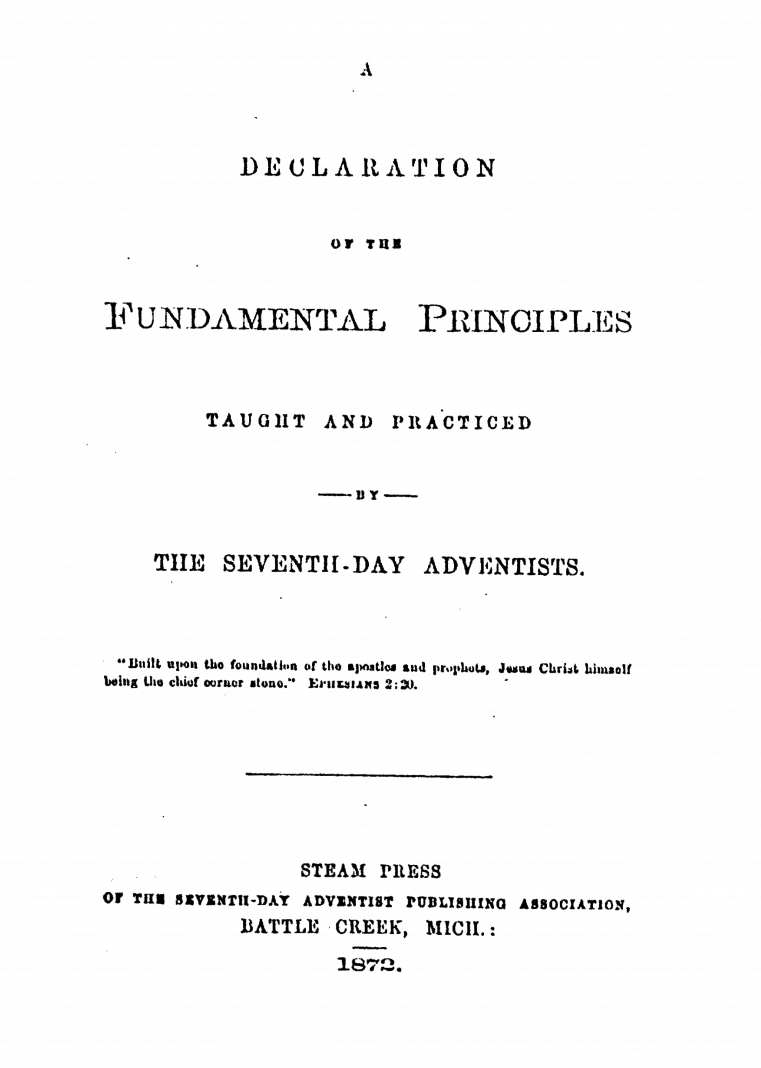
\includegraphics[width=1\linewidth]{images/declaration-of-the-fundamental-principles.PNG}
    \caption*{Scan of the Declaration of the Fundamental Principles, 1872.}
    \label{fig:declaration-of-the-fundamental-principles}
\end{figure}


\begin{figure}
    \centering
    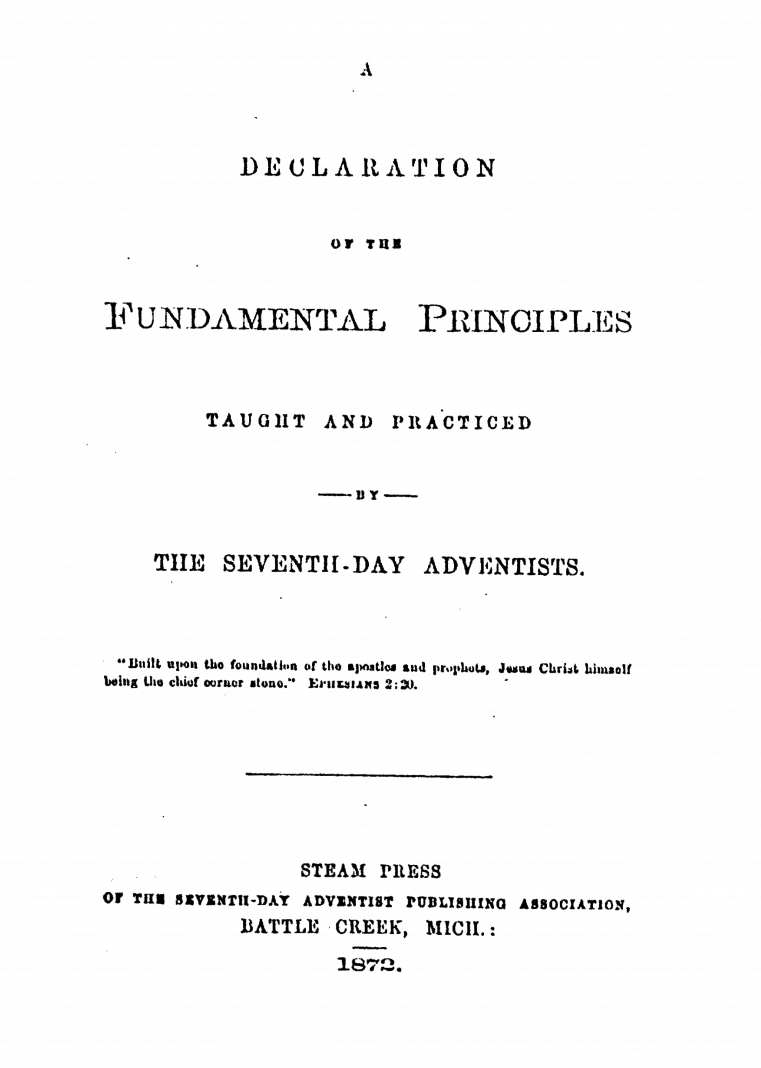
\includegraphics[width=1\linewidth]{images/declaration-of-the-fundamental-principles.PNG}
    \caption*{Scan de la Déclaration des Principes Fondamentaux, 1872.}
    \label{fig:declaration-of-the-fundamental-principles}
\end{figure}


\others{In presenting to the \textbf{public} this \textbf{synopsis of our faith}, we wish to have it distinctly understood that \textbf{we have no articles of faith, creed, or discipline, }\textbf{\underline{aside from the Bible}}. We \textbf{do not} put forth this as \textbf{having any authority with our people}, \textbf{nor is it designed to secure uniformity among them}, \textbf{as a system of faith}, \textbf{but is a brief statement of \underline{what is, and has been, with great unanimity, held by them}}. We often find it necessary to meet inquiries on this subject, and sometimes to correct false statements circulated against us, and to remove erroneous impressions which have obtained with those who have not had an opportunity to become acquainted with our faith and practice. Our only object is to meet this necessity.}


\others{En présentant au \textbf{public} ce \textbf{synopsis de notre foi}, nous souhaitons qu'il soit clairement compris que \textbf{nous n'avons pas d'articles de foi, de credo ou de discipline, }\textbf{\underline{en dehors de la Bible}}. Nous \textbf{ne} présentons pas ceci comme \textbf{ayant une quelconque autorité sur notre peuple}, \textbf{ni n'est-il conçu pour assurer l'uniformité parmi eux}, \textbf{comme un système de foi}, \textbf{mais c'est une brève déclaration de \underline{ce qui est, et a été, avec une grande unanimité, soutenu par eux}}. Nous trouvons souvent nécessaire de répondre aux questions sur ce sujet, et parfois de corriger de fausses déclarations diffusées contre nous, et d'éliminer les impressions erronées qui ont été obtenues par ceux qui n'ont pas eu l'occasion de se familiariser avec notre foi et notre pratique. Notre seul objectif est de répondre à cette nécessité.}


\othersnogap{\textbf{As Seventh-day Adventists we desire simply that our position shall be understood}; and we are the more solicitous for this because there are many who call themselves Adventists who hold views with which we can have no sympathy, some of which, we think, are subversive of the plainest and most important principles set forth in the word of God...}[The Fundamental Principles 1872, p. 3.1][https://egwwritings.org/read?panels=p928.8]


\othersnogap{\textbf{En tant qu'Adventistes du Septième Jour, nous désirons simplement que notre position soit comprise}; et nous sommes d'autant plus soucieux de cela parce qu'il y a beaucoup de personnes qui se disent Adventistes qui soutiennent des points de vue avec lesquels nous ne pouvons avoir aucune sympathie, dont certains, nous pensons, sont subversifs des principes les plus simples et les plus importants énoncés dans la parole de Dieu...}[Les Principes Fondamentaux 1872, p. 3.1][https://egwwritings.org/read?panels=p928.8]


This synopsis of faith consisted of 25 points, which represented \others{what is, and has been, with great unanimity, held by} Seventh-day Adventists. These 25 points constituted \egwinline{\textbf{the foundation} that was \textbf{laid at the beginning} of our work \textbf{by prayerful study} of the word and by revelation}. In 1904, Sister White told us that \egwinline{upon \textbf{this foundation} we have been building for \textbf{the past fifty years}.} These are the \egwinline{\textbf{the fundamental principles that are based upon unquestionable authority}}, that God \egwinline{calls upon us to \textbf{hold firmly}, with the grip of faith}. In other words, she repeated, \egwinline{we are to \textbf{hold to the sure pillars of our faith}}.


Ce synopsis de foi consistait en 25 points, qui représentaient \others{ce qui est, et a été, avec une grande unanimité, soutenu par} les Adventistes du Septième Jour. Ces 25 points constituaient \egwinline{\textbf{la fondation} qui a été \textbf{posée au début} de notre œuvre \textbf{par l'étude priante} de la parole et par révélation}. En 1904, Sœur White nous a dit que \egwinline{sur \textbf{cette fondation} nous avons construit pendant \textbf{les cinquante dernières années}.} Ce sont \egwinline{\textbf{les principes fondamentaux qui sont basés sur une autorité incontestable}}, que Dieu \egwinline{nous appelle à \textbf{tenir fermement}, avec la poigne de la foi}. En d'autres termes, elle a répété, \egwinline{nous devons \textbf{nous tenir aux piliers sûrs de notre foi}}.


In 1904, Sister White wrote about\egwinline{the \textbf{efforts of the enemy to undermine the foundation of our faith}}. She wrote about the movement that would\egwinline{consist in \textbf{giving up} the doctrines which stand as \textbf{the pillars of our faith}}. This reformation, if accepted, would discard\egwinline{\textbf{the principles of truth} that God in His wisdom has given to the remnant church} and\egwinline{\textbf{the fundamental principles} that have sustained the work for the last fifty years \textbf{would be accounted as error}}. This movement started about the time when Dr. John H. Kellogg published the book, “Living Temple”.


En 1904, Sœur White a écrit à propos des\egwinline{\textbf{efforts de l'ennemi pour saper la fondation de notre foi}}. Elle a écrit sur le mouvement qui\egwinline{consisterait à \textbf{abandonner} les doctrines qui se tiennent comme \textbf{les piliers de notre foi}}. Cette réforme, si acceptée, rejetterait\egwinline{\textbf{les principes de vérité} que Dieu dans Sa sagesse a donnés à l'église du reste} et\egwinline{\textbf{les principes fondamentaux} qui ont soutenu l'œuvre pendant les cinquante dernières années \textbf{seraient considérés comme une erreur}}. Ce mouvement a commencé à peu près au moment où le Dr John H. Kellogg a publié le livre, “Le Temple Vivant”.


\egw{About the time that ‘Living Temple’ was published, there passed before me in the night season, \textbf{representations indicating that some danger was approaching}, and that I must prepare for it by \textbf{writing out the things} God has revealed to me \textbf{regarding \underline{the foundation principles of our faith}}.}[SpTB02 52.3; 1904][https://egwwritings.org/read?panels=p417.267]


\egw{À peu près au moment où ‘Le Temple Vivant’ a été publié, il est passé devant moi pendant la nuit, \textbf{des représentations indiquant qu'un danger approchait}, et que je devais m'y préparer en \textbf{écrivant les choses} que Dieu m'a révélées \textbf{concernant \underline{les principes fondamentaux de notre foi}}.}[SpTB02 52.3; 1904][https://egwwritings.org/read?panels=p417.267]


By publishing “Living Temple”, \textbf{foundation principles of our faith} \textbf{would be undermined}\egwinline{through the dissemination of \textbf{seductive theories}} contained therein.


En publiant “Le Temple Vivant”, \textbf{les principes fondamentaux de notre foi} \textbf{seraient sapés}\egwinline{par la diffusion de \textbf{théories séduisantes}} contenues dans celui-ci.


\egw{I have been instructed by the heavenly messenger that some of the reasoning in the book, ‘Living Temple,’ is unsound and that \textbf{this reasoning would lead astray} the minds of those who are not thoroughly established on \textbf{the foundation principles} of present truth. It introduces that which is naught but speculation in \textbf{regard to \underline{the personality of God and where His presence is}}.}[SpTB02 51.3; 1904][https://egwwritings.org/read?panels=p417.262]


\egw{J'ai reçu l'instruction du messager céleste que certains des raisonnements dans le livre ‘Le Temple Vivant’ sont erronés et que \textbf{ce raisonnement égarerait} les esprits de ceux qui ne sont pas fermement établis sur \textbf{les principes fondamentaux} de la vérité présente. Il introduit ce qui n'est que spéculation en \textbf{ce qui concerne \underline{la personnalité de Dieu et où est Sa présence}}.}[SpTB02 51.3; 1904][https://egwwritings.org/read?panels=p417.262]


Sister White is very particular in pointing out that the reasoning contained in the book Living Temple,\egwinline{\textbf{would lead astray}} from the\egwinline{\textbf{the foundation principles} of present truth}. These reasonings are in\egwinline{\textbf{regard to the personality of God and where His presence is}}.


Sœur White est très précise en soulignant que le raisonnement contenu dans le livre Le Temple Vivant,\egwinline{\textbf{égarerait}} des\egwinline{\textbf{les principes fondamentaux} de la vérité présente}. Ces raisonnements concernent\egwinline{\textbf{la personnalité de Dieu et où est Sa présence}}.


As mentioned before, the word ‘\textit{personality’}, in the context of the nineteenth century, is defined as “\textit{the quality or state of being a person}”\footnote{\href{https://www.merriam-webster.com/dictionary/personality}{Merriam-Webster Dictionary}, word ‘\textit{personality}’}. In other words, this term conveys the answer to the question, “\textit{what is it that defines someone to be a person?}”, “\textit{What is the quality or state of someone being a person?}” In the case of the \emcap{personality of God}, the question is, “\textit{Is God a person and what is it that defines Him as being a person? What is the quality or state of God being a person?}”


Comme mentionné précédemment, le mot ‘\textit{personnalité}’, dans le contexte du dix-neuvième siècle, est défini comme “\textit{La qualité ou l'état par lequel quelqu'un est défini comme une personne}”\footnote{\href{https://www.merriam-webster.com/dictionary/personality}{Merriam-Webster Dictionary}, mot ‘\textit{personnalité}’}. En d'autres termes, ce terme répond à la question, “\textit{qu'est-ce qui définit quelqu'un comme étant une personne ?}”, “\textit{Quelle est la qualité ou l'état de quelqu'un étant une personne ?}” Dans le cas de la \emcap{personnalité de Dieu}, la question est, “\textit{Dieu est-il une personne et qu'est-ce qui le définit comme étant une personne ? Quelle est la qualité ou l'état de Dieu comme étant une personne ?}”


The reasoning of Dr. Kellogg regarding these questions expressed in the book Living Temple, is\egwinline{unsound}. The sentiments, in\egwinline{\textbf{regard to the personality of God and where His presence is}},\egwinline{advocated in the book, did not bear the indorsement of God, and that they were \textbf{a snare that the enemy had prepared for the last days}}. As we are living in the last days, we ought to ask ourselves these questions. Likewise, we are to question the biblical validity of the statements in the \emcap{Fundamental Principles} regarding the \emcap{personality of God} and where His presence is. How do the \emcap{Fundamental Principles} define God as being a person, and what do they say regarding God’s presence?


Le raisonnement du Dr. Kellogg concernant ces questions exprimées dans le livre Le Temple Vivant, est\egwinline{erroné}. Le raisonnement, en\egwinline{\textbf{ce qui concerne la personnalité de Dieu et où est Sa présence}},\egwinline{préconisé dans le livre, ne portait pas l'approbation de Dieu, et c'était \textbf{un piège que l'ennemi avait préparé pour les derniers jours}}. Comme nous vivons dans les derniers jours, nous devrions nous poser ces questions. De même, nous devons questionner la validité biblique des déclarations dans les \emcap{Principes Fondamentaux} concernant la \emcap{personnalité de Dieu} et où est Sa présence. Comment les \emcap{Principes Fondamentaux} définissent-ils Dieu comme étant une personne, et que disent-ils concernant la présence de Dieu ?


The first point listed below deals with the \emcap{personality of God} and His presence. The second point gives the context to the first. Please consider a few questions while reading them: Who is referred to as one God? How is God defined as a person or in other words, what is the quality or state of Him being a person? How do these points talk about the presence of God?


Le premier point énuméré ci-dessous traite de la \emcap{personnalité de Dieu} et de Sa présence. Le deuxième point donne le contexte au premier. Veuillez considérer quelques questions en les lisant : Qui est désigné comme un seul Dieu ? Comment Dieu est-il défini comme une personne ou en d'autres termes, quelle est la qualité ou l'état de Lui étant une personne ? Comment ces points parlent-ils de la présence de Dieu ?


\others{“I – That there is \textbf{one God}, \textbf{\underline{a personal, spiritual being}}, \textbf{the creator of all things}, omnipotent, omniscient, and eternal, infinite in wisdom, holiness, justice, goodness, truth, and mercy; unchangeable, and \textbf{\underline{everywhere present by his representative, the Holy Spirit}}. Ps. 139:7.”}


\others{“I – Qu'il y a \textbf{un seul Dieu}, \textbf{\underline{un être personnel et spirituel}}, \textbf{le créateur de toutes choses}, omnipotent, omniscient, et éternel, infini en sagesse, sainteté, justice, bonté, vérité et miséricorde ; immuable, et \textbf{\underline{présent partout par son représentant, le Saint-Esprit}}. Ps. 139:7.”}


\othersnogap{II – That there is \textbf{one Lord Jesus Christ, }\textbf{\underline{the Son of the Eternal Father}}, the one \textbf{\underline{by}}\textbf{ whom God created all things}, and by whom they do consist; …”}[The Fundamental Principles 1889, point no. 1.,2.,.] \footnote{See \hyperref[chap:appendix]{Appendix} for the full list of the Fundamental Principles} \footnote{From 1872 until 1914, the Fundamental Principles remained constant and unchanged, with the exception in 1889, when James Smith added three new points. But during all those years, the points concerning “\textit{the personality of God}” and “\textit{where His presence is}” remained the same. }


\othersnogap{II – Qu'il y a \textbf{un seul Seigneur Jésus-Christ, }\textbf{\underline{le Fils du Père Éternel}}, celui \textbf{\underline{par}}\textbf{ qui Dieu a créé toutes choses}, et par qui elles subsistent ; …“}[Les Principes Fondamentaux 1889, point no. 1.,2.,.] \footnote{Voir \hyperref[chap:appendix]{Annexe} pour la liste complète des Principes Fondamentaux} \footnote{De 1872 jusqu'à 1914, les Principes Fondamentaux sont restés constants et inchangés, à l'exception de 1889, lorsque James Smith a ajouté trois nouveaux points. Mais durant toutes ces années, les points concernant “\textit{la personnalité de Dieu}” et “\textit{où est Sa présence}” sont restés les mêmes. }


In the time of Ellen White, Seventh-day Adventists believed in one God—a personal, spiritual being, the Creator of all things—and they believed that this God created everything by His Son Jesus Christ. They addressed the Father as one God, and they addressed Christ as the Son of God. The quality or state of God being a person is expressed in the term “\textit{personal, spiritual being}”. Regarding His presence, the \emcap{Fundamental Principles} state that He is everywhere present by His representative, the Holy Spirit. The meaning of these principles requires very special attention. Keeping within the historical context, this will be the subject of our following studies.


À l'époque d'Ellen White, les Adventistes du Septième Jour croyaient en un seul Dieu—un être personnel et spirituel, le Créateur de toutes choses—et ils croyaient que ce Dieu avait tout créé par Son Fils Jésus-Christ. Ils s'adressaient au Père comme étant un seul Dieu, et ils s'adressaient au Christ comme étant le Fils de Dieu. La qualité ou l'état de Dieu comme étant une personne est exprimé dans le terme “\textit{être personnel et spirituel}”. Concernant Sa présence, les \emcap{Principes Fondamentaux} déclarent qu'Il est présent partout par Son représentant, le Saint-Esprit. La signification de ces principes requiert une attention très particulière. En restant dans le contexte historique, ce sera le sujet de nos études suivantes.


\section*{The Test}


\section*{Le Test}


Most obviously, these \emcap{fundamental principles} do not contain the doctrine of the Trinity! More precisely, the sentiments “\textit{three in one},” or “\textit{one in three}”, in reference to God, are nowhere to be found—which are present in today’s \textit{Fundamental Beliefs}. Only the Father is referred to as “\textit{one God’‘}. But before rushing to swift conclusions, and condemning the doctrine of the Trinity as\egwinline{\textbf{seductive theories,}} which\egwinline{\textbf{undermine the foundation of our faith}}, please bear in mind that Sister White presents a comprehensive list of characteristics that must be fulfilled in order for it to be deemed as such.


De toute évidence, ces \emcap{principes fondamentaux} ne contiennent pas la doctrine de la Trinité ! Plus précisément, les raisonnements “\textit{trois en un},” ou “\textit{un en trois}”, en référence à Dieu, ne se trouvent nulle part—qui sont présents dans les \textit{Croyances Fondamentales} d'aujourd'hui. Seul le Père est désigné comme “\textit{un seul Dieu’‘}. Mais avant de se précipiter vers des conclusions hâtives, et de condamner la doctrine de la Trinité comme\egwinline{\textbf{des théories séduisantes,}} qui\egwinline{\textbf{sapent le fondement de notre foi}}, veuillez garder à l'esprit que Sœur White présente une liste complète de caractéristiques qui doivent être remplies pour qu'elle soit considérée comme telle.


If the Trinity doctrine is questionable, then the trinitarian sentiments would need to:
\begin{itemize}
    \item rob the people of God of their past experience
    \item destroy the \emcap{personality of God}
    \item tear down the pillars of our faith or lead astray from the foundation principles
    \item be presented as if Mrs. White supported them
\end{itemize}


Si la doctrine de la Trinité est discutable, alors le raisonnement trinitaire devrait :
\begin{itemize}
    \item priver le peuple de Dieu de son expérience passée
    \item détruire la \emcap{personnalité de Dieu}
    \item démolir les piliers de notre foi ou détourner des principes fondamentaux
    \item être présenté comme si Mme White les soutenait
\end{itemize}


It is not our intention to deal with any of Kellogg’s seductive theories, but rather to study the \emcap{personality of God} in its historical background. As we do this, we will face the evidence of Sister White reactively warning the church of these characteristics.


Notre intention n'est pas de traiter des théories séductrices de Kellogg, mais plutôt d'étudier la \emcap{personnalité de Dieu} dans son contexte historique. Ce faisant, nous ferons face aux preuves que Sœur White mettait en garde l'église de manière réactive contre ces caractéristiques.


% The Fundamental Prinicples

\begin{titledpoem}
    \stanza{
        The Masterworker built a foundation strong, \\
        To guide God's people as they journey long. \\
        These truths revealed through prayer and earnest toil, \\
        Stand firm on heaven's unquestionable soil.
    }

    \stanza{
        God as one personal and spiritual being, \\
        Present through His Spirit, all-knowing, all-seeing. \\
        Christ as the Son of the Eternal Father, \\
        These pillars of faith we should hold, not bother.
    }

    \stanza{
        When men depart from these principles true, \\
        Undermining foundations through teachings new, \\
        The wisdom of ages they quickly discard, \\
        And God's revealed pathway becomes sadly marred.
    }

    \stanza{
        Hold firmly the truth with unwavering grip, \\
        Let not from these anchors your faith ever slip. \\
        For what God established through pioneers' hands, \\
        Through tempest and storm eternally stands.
    }
\end{titledpoem}